\documentclass[a4paper,english]{ifimaster}

\usepackage[utf8]{inputenc}
\usepackage{babel,duomasterforside}
\usepackage{hyperref}
\usepackage{pdfsync}
\usepackage{csquotes}
\usepackage{graphicx}
\usepackage{minted}
\usepackage{varioref}
\usepackage{parskip}
\usepackage[backend=biber]{biblatex}

\addbibresource{citations.bib}
\graphicspath{ {./illustrations/} }

\newcommand{\todo}[1]{\textcolor{red}{[[TODO: #1]]}\PackageWarning{TODO:}{#1!}}

\title{Three Way Merge for Feature Model Evolution Plans}
\date{May 2021}
\author{Eirik Halvard Sæther}
\synctex=1

\begin{document}

\duoforside[dept={Department of Informatics},
program={Informatics: Programming and Systems Architecture},
long]
\frontmatter{}

\chapter*{Acknowledgements}

Thanks to Ida

Thanks to Ingrid and Crystal

Thanks to Germans, everyone on the LTEP project for input etc.

\newpage
\thispagestyle{empty}
\mbox{}
\chapter*{Abstract}

\todo{write abstract}

Feature Model Evolution Plans is intended to help ease the development of software product lines (SPLs). Feature Models allow software engineers to explicitly encode the similarities and differences of an SPL. However, due to the changing nature of an SPL, Evolution Plans allows for representing the \textit{evolution} of a feature model, not just the feature model as a single point in time.

Evolution planning of an SPL is often a dynamic, changing process, due to changing demands of the focus of development. The evolution planning is often not just done by a single engineer, but multiple engineers, working separately and independent of each other. Due to these factors, the need to unify and synchronize the changes the evolution plan emerges.

In this thesis, we develop a merge tool for Feature Model Evolution Plans. The core of the tool is a three-way merge algorithm. Given two different versions of an evolution plan, together with the common evolution plan they were derived from, the merge algorithm will attempt to merge all the different changes from both versions. If the merges are unifiable, the algorithm will succeed and yield the merged result containing the changes from both versions. However, if the changes are conflicting in any way, breaking the structure or semantics of evolution plans, the algorithm will stop, telling the user the reason of failure.

\tableofcontents{}
\listoffigures{}
\listoftables{}

\chapter*{Preface}

\todo{write better and more}
something about the LTEP project

something about summer project?

\mainmatter{}
\chapter{Introduction}%
\label{cha:introduction}

\section{Chapter Overview}%
\label{sec:chapter_overview}

\section{Project Source Code}%
\label{sec:project_source_code}

\chapter{Background}%
\label{cha:background}

\section{Software Product Lines}%
\label{sec:software_product_lines}

\section{Evolution Planning}%
\label{sec:evolution_planning}

\section{Haskell and Algebraic Data Types}%
\label{sec:haskell_and_algebraic_data_types}

\chapter{Formal Semantics of Feature Model Evolution Plans}%
\label{cha:formal_semantics_of_feature_model_evolution_plans}

\chapter{Three Way Merge Algorithm}%
\label{cha:three_way_merge_algorithm}

\section{Algorithm Overview}%
\label{sec:algorithm_overview}

\subsection{Three-Way Merging of Evolution Plans}%
\label{sub:three_way_merging_of_evolution_plans}

The three-way merge algorithm for feature model evolution plans will take two different versions of an evolution plan, \textit{version 1} and \textit{version 2}, and attempt to merge the evolution plans into a single plan. In order to do so, a third evolution plan has to be provided, which is the common evolution plan they were derived from. The common evolution plan, called \textit{base}, will implicitly provide information about what things were added, removed and changed in each of the derived evolution plans.

\subsection{Soundness Assumption}%
\label{sub:soundness_assumption}

The three-way merge algorithm will assume that the three evolution plans provided are sound. By assuming the soundness of the plans, the algorithm can leverage this to create a better merge result. But more importantly, the assumption is based around the fact that there is no point in merging an evolution plan you know violates soundness in some way.

\subsection{Algorithm Phases}%
\label{sub:algorithm_phases}

In order to merge the different versions of the evolution plan, the algorithm is separated into several distinct phases. The different steps and phases of the algorithm can be seen in Figure~\ref{fig:merge_outline}.

\begin{figure}[htbp]
  \centering
  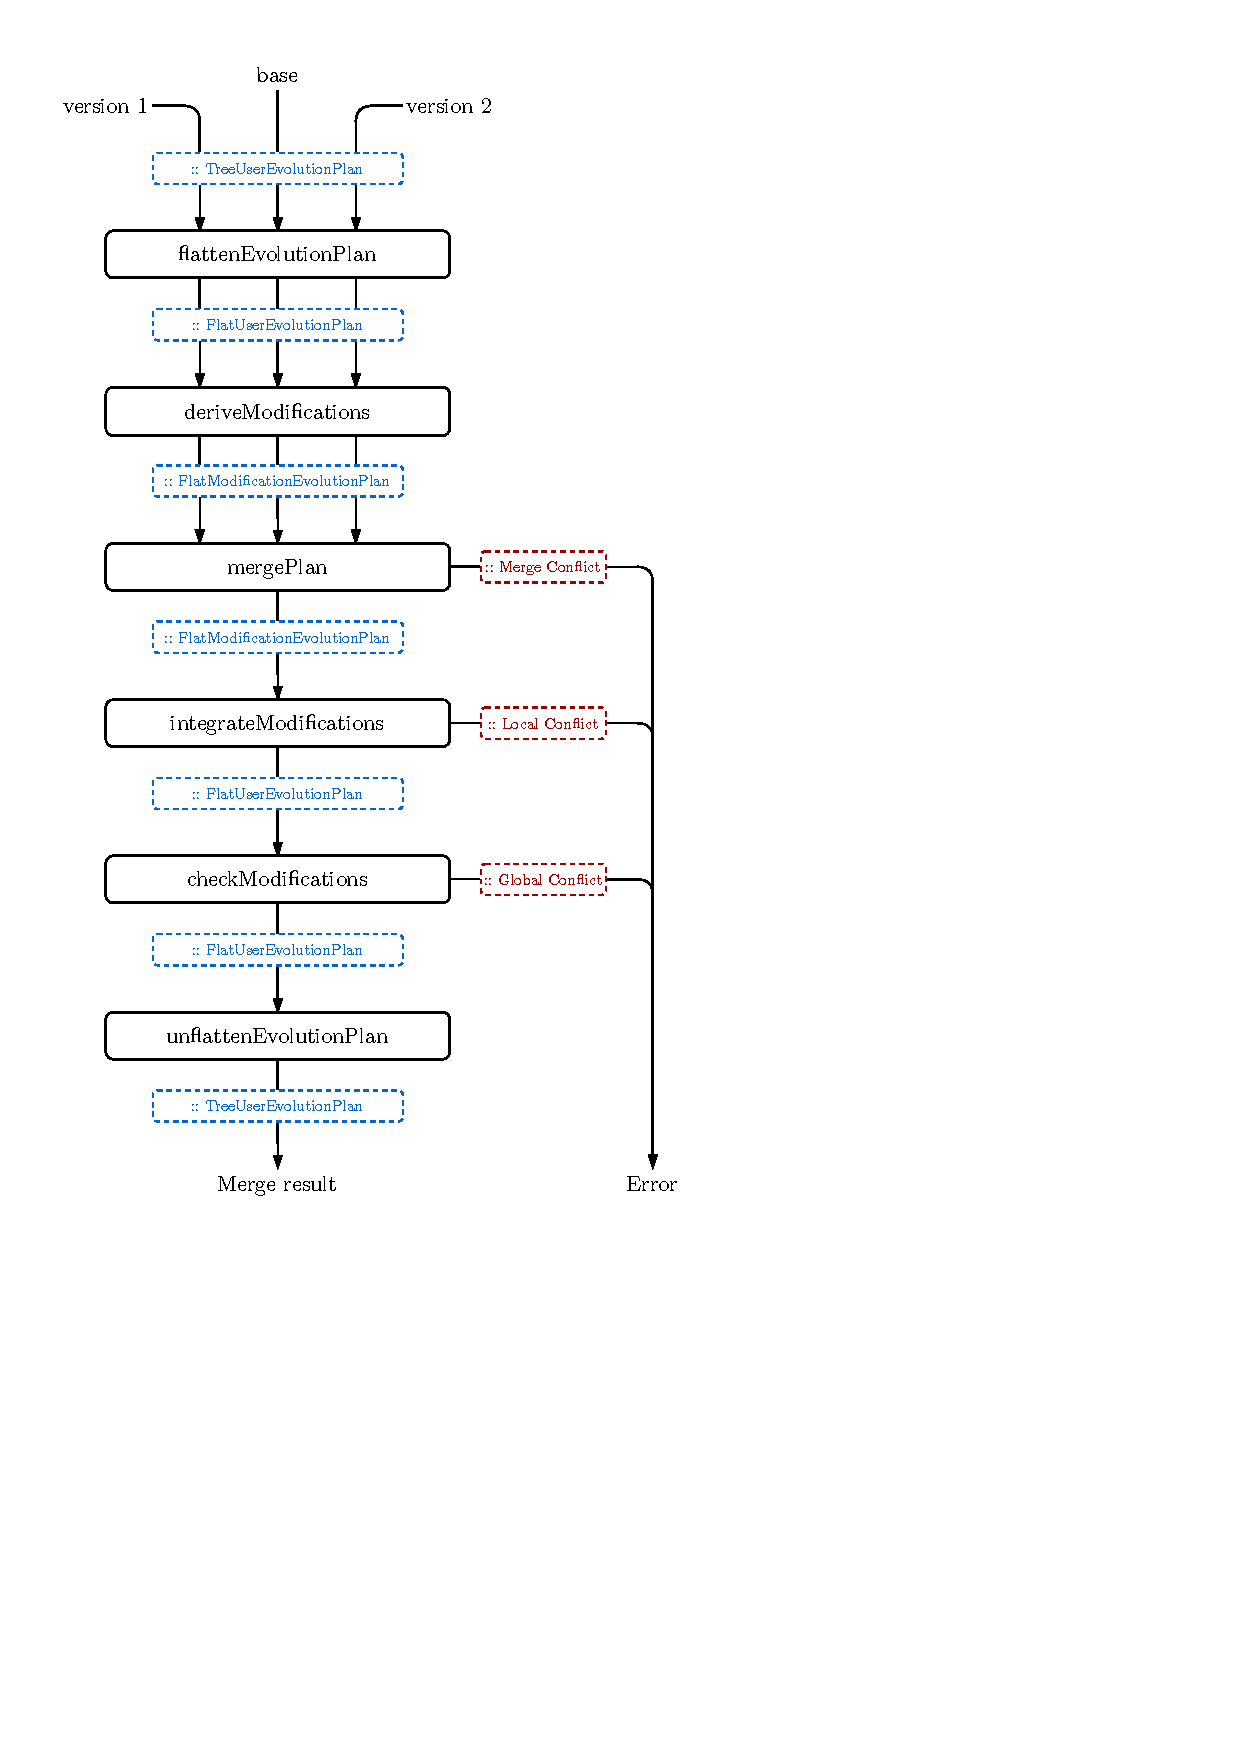
\includegraphics[width=0.8\linewidth]{merge_outline}
  \caption{Outline of the three-way merge algorithm}%
  \label{fig:merge_outline}
\end{figure}

The first phase is transforming the three different evolution plans into representations that is more suitable for merging. This includes converting both the way feature models are represented as well as the way the entire evolution plan is represented. This phase includes the \texttt{flattenEvolutionPlan} and \texttt{deriveModifications}, which is described in further detail in \vref{sec:converting_to_a_suitable_representation}

After changing the way evolution plans are represented, the second phase of the algorithm will calculate the differences between the \textit{base} evolution plan and both derived evolution plans, \textit{version 1}, and \textit{version 2}. This will let us know what were added, changed and removed in each of the derived evolution plans. This phase is part of the \texttt{mergePlan} function, which is described in further detail in \vref{sec:detecting_the_changes_between_versions}

The information from the previous phase will be used to create a single merged evolution plan. This evolution plan is simply just the \textit{base} evolution plan integrated with all the changes from \textit{version 1} and \textit{version 2}. This phase is part of the \texttt{mergePlan} function, which is described in further detail in \vref{sec:merging_intended_changes}

Now that a single merged evolution plan is provided, the last step is to ensure that the plan is following the structural and semantic requirements of an evolution plan. Merging all changes from both versions might yield various inconsistencies. This includes structural conflicts such as orphan features, entire subtrees forming cycles, removing non-empty features, etc. The last phase includes converting back to the original representation, as well as ensuring soundness while doing so. This phase is part of the \texttt{integrateModifications}, \texttt{checkModifications} and \texttt{unflattenEvolutionPlan} functions, which is explained further in \vref{sec:ensuring_structural_and_semantic_soundness_of_merge_result}

\subsection{Conflicts}%
\label{sub:conflicts}

During the different phases of the merge algorithm, different kind of conflicts or errors could occur. Depending on what part of the algorithm a conflict occurred, the conflicts might be either a \textit{merge}, \textit{local} or \textit{global} conflict. For example, if both versions perform different operations on the same feature at the same time point, the 

\section{Converting To a Suitable Representation}%
\label{sec:converting_to_a_suitable_representation}

\subsection{Representing Feature Models}%
\label{sub:representing_feature_models}

\subsection{Representing Evolution Plans}%
\label{sub:representing_evolution_plans}

\section{Detecting the Changes Between Versions}%
\label{sec:detecting_the_changes_between_versions}

\section{Merging Intended Changes}%
\label{sec:merging_intended_changes}

\section{Ensuring structural and semantic soundness of the merge result}%
\label{sec:ensuring_structural_and_semantic_soundness_of_merge_result}

\chapter{Conclusion and Future Work}%
\label{cha:conclusion_and_future_work}

\backmatter{}

\printbibliography

\end{document}
